\documentclass[12pt]{article}

\usepackage[a4paper,margin=1in]{geometry}
\usepackage{amsmath,amssymb}
\usepackage{newtxtext,newtxmath}
\usepackage{fancyhdr}
\usepackage{listings}
\usepackage{graphicx}
\usepackage{float}
\usepackage{hyperref}
\usepackage{booktabs}
\usepackage{xcolor}

\setlength{\parindent}{0pt}
\setlength{\parskip}{5pt}

% Keep entire document at 12 pt
\AtBeginDocument{
    \fontsize{12pt}{14pt}\selectfont
}

% ------------------------------------------------
% Header Configuration
% ------------------------------------------------
\pagestyle{fancy}
\fancyhf{}
\fancyhead[L]{Name: \underline{Shaik Jnaved}}
\fancyhead[R]{Enrollment No.: \underline{P26DS001}}
\renewcommand{\headrulewidth}{0.4pt}
\setlength{\headheight}{15pt}

% ------------------------------------------------
% Code Formatting Configuration
% ------------------------------------------------
\lstset{
    basicstyle=\ttfamily\fontsize{8.5pt}{10.5pt}\selectfont,
    breaklines=true,
    frame=single,
    columns=fullflexible,
    keepspaces=true,
    showstringspaces=false,
    keywordstyle=\color{blue}\bfseries,
    commentstyle=\color{gray}\itshape,
    stringstyle=\color{teal}
}

\begin{document}

% ==============================================================================
% TITLE BANNER
% ==============================================================================
\begin{center}
\textbf{\Large SARDAR VALLABHBHAI NATIONAL INSTITUTE OF TECHNOLOGY, SURAT}\\[4pt]
\textbf{\large Department of Computer Science \& Engineering}\\[3pt]
\textbf{\large CS103 / CSDS103: Design and Analysis of Algorithms}\\[3pt]
\textbf{\large M.Tech. (DS) I Year -- Semester I}\\[4pt]
\textbf{\Large Lab Assignment 6: Comprehensive Laboratory Report}
\end{center}

\vspace{0.2cm}
\hrule
\vspace{0.4cm}

\textbf{Overview}:\\
This laboratory report details seven algorithmic problems spanning the Divide and Conquer paradigm, computational geometry, empirical timing analysis, sorting partition strategies, multi-dimensional search routines, and theoretical systems architecture:
\begin{itemize}
    \item \textbf{Assignment 1}: Divide-and-Conquer Algorithm for Binary Tree Levels
    \item \textbf{Assignment 2}: Inversion Counting: Brute Force $\mathcal{O}(n^2)$ vs. Merge Sort $\mathcal{O}(n \log n)$
    \item \textbf{Assignment 3}: Quicksort Partition Routines: Lomuto (Textbook) vs. Hoare (Class)
    \item \textbf{Assignment 4}: Two-Dimensional Convex Hull Construction
    \item \textbf{Assignment 5}: Shortest Distance Between Two Points in 3D Euclidean Space
    \item \textbf{Assignment 6}: Infeasibility of Pure Empirical Analysis for Algorithmic Comparison
    \item \textbf{Assignment 7}: Generalized Two-Dimensional Peak Finding in $\mathcal{O}(n \log m)$ Time
\end{itemize}

\vspace{0.3cm}

% ==============================================================================
% ASSIGNMENT 1: TREE LEVELS
% ==============================================================================
\section*{Assignment 1: Divide-and-Conquer Binary Tree Level Computation}

\subsection*{1.1 Problem Statement and Algorithmic Design}
\textbf{Task}: Design a divide-and-conquer algorithm for computing the number of levels (height) in a binary tree such that:
\begin{itemize}
    \item The algorithm returns $0$ for an empty tree (\texttt{root is None}).
    \item The algorithm returns $1$ for a single-node tree (\texttt{root.left is None and root.right is None}).
\end{itemize}

\textbf{Divide-and-Conquer Formulation}:
\begin{enumerate}
    \item \textbf{Base Cases}:
    \begin{itemize}
        \item If $\text{root} = \text{null}$, return $0$.
        \item If $\text{root.left} = \text{null}$ and $\text{root.right} = \text{null}$, return $1$.
    \end{itemize}
    \item \textbf{Divide}: Recursively compute the number of levels in the left and right subtrees:
    \[
    L = \text{compute\_levels}(\text{root.left}), \quad R = \text{compute\_levels}(\text{root.right})
    \]
    \item \textbf{Combine}: The number of levels for the current root is:
    \[
    \text{levels}(\text{root}) = 1 + \max(L, R)
    \]
\end{enumerate}

\subsection*{1.2 Time Efficiency Class Analysis}
Let $N$ be the total number of nodes in the binary tree.
At each node, the algorithm performs a constant number of operations: two null-pointer checks, two recursive invocations, a maximum comparison, and an addition ($\Theta(1)$ work per node).
The recurrence relation for a tree with $k$ nodes in the left subtree and $N - 1 - k$ nodes in the right subtree is:
\[
T(N) = T(k) + T(N - 1 - k) + c, \quad T(0) = d_0, \quad T(1) = d_1
\]
Summing over all $N$ nodes, every node is visited exactly once. Hence:
\[
T(N) = \Theta(N)
\]
\textbf{Auxiliary Space Complexity}: $\mathcal{O}(H)$, where $H$ is the height of the tree, representing the recursion stack frame depth ($\mathcal{O}(\log N)$ for balanced trees, $\mathcal{O}(N)$ for skewed trees).

\subsection*{1.3 Python Implementation (\texttt{tree\_levels.py})}
\begin{lstlisting}[language=Python]
class TreeNode:
    def __init__(self, val: int = 0, left=None, right=None):
        self.val = val
        self.left = left
        self.right = right

def compute_levels(root: TreeNode | None) -> int:
    if root is None:
        return 0
    if root.left is None and root.right is None:
        return 1
    left_levels = compute_levels(root.left)
    right_levels = compute_levels(root.right)
    return 1 + max(left_levels, right_levels)
\end{lstlisting}

\subsection*{1.4 Empirical Timing Results \& Comparison}
We benchmarked the algorithm over $200,000$ iterations on empty, 1-level, 2-level, and 3-level binary trees.

\begin{table}[H]
\centering
\caption{Empirical Execution Times for Binary Tree Level Computation.}
\label{tab:tree_levels}
\vspace{0.2cm}
\begin{tabular}{lccc}
\toprule
\textbf{Tree Structure} & \textbf{Node Count ($N$)} & \textbf{Expected Levels} & \textbf{Average Time (ns)} \\
\midrule
Empty Tree   & 0 & 0 & 28.55 \\
One-level    & 1 & 1 & 41.45 \\
Two-level    & 3 & 2 & 140.76 \\
Three-level  & 7 & 3 & 340.51 \\
\bottomrule
\end{tabular}
\end{table}

\begin{figure}[H]
\centering
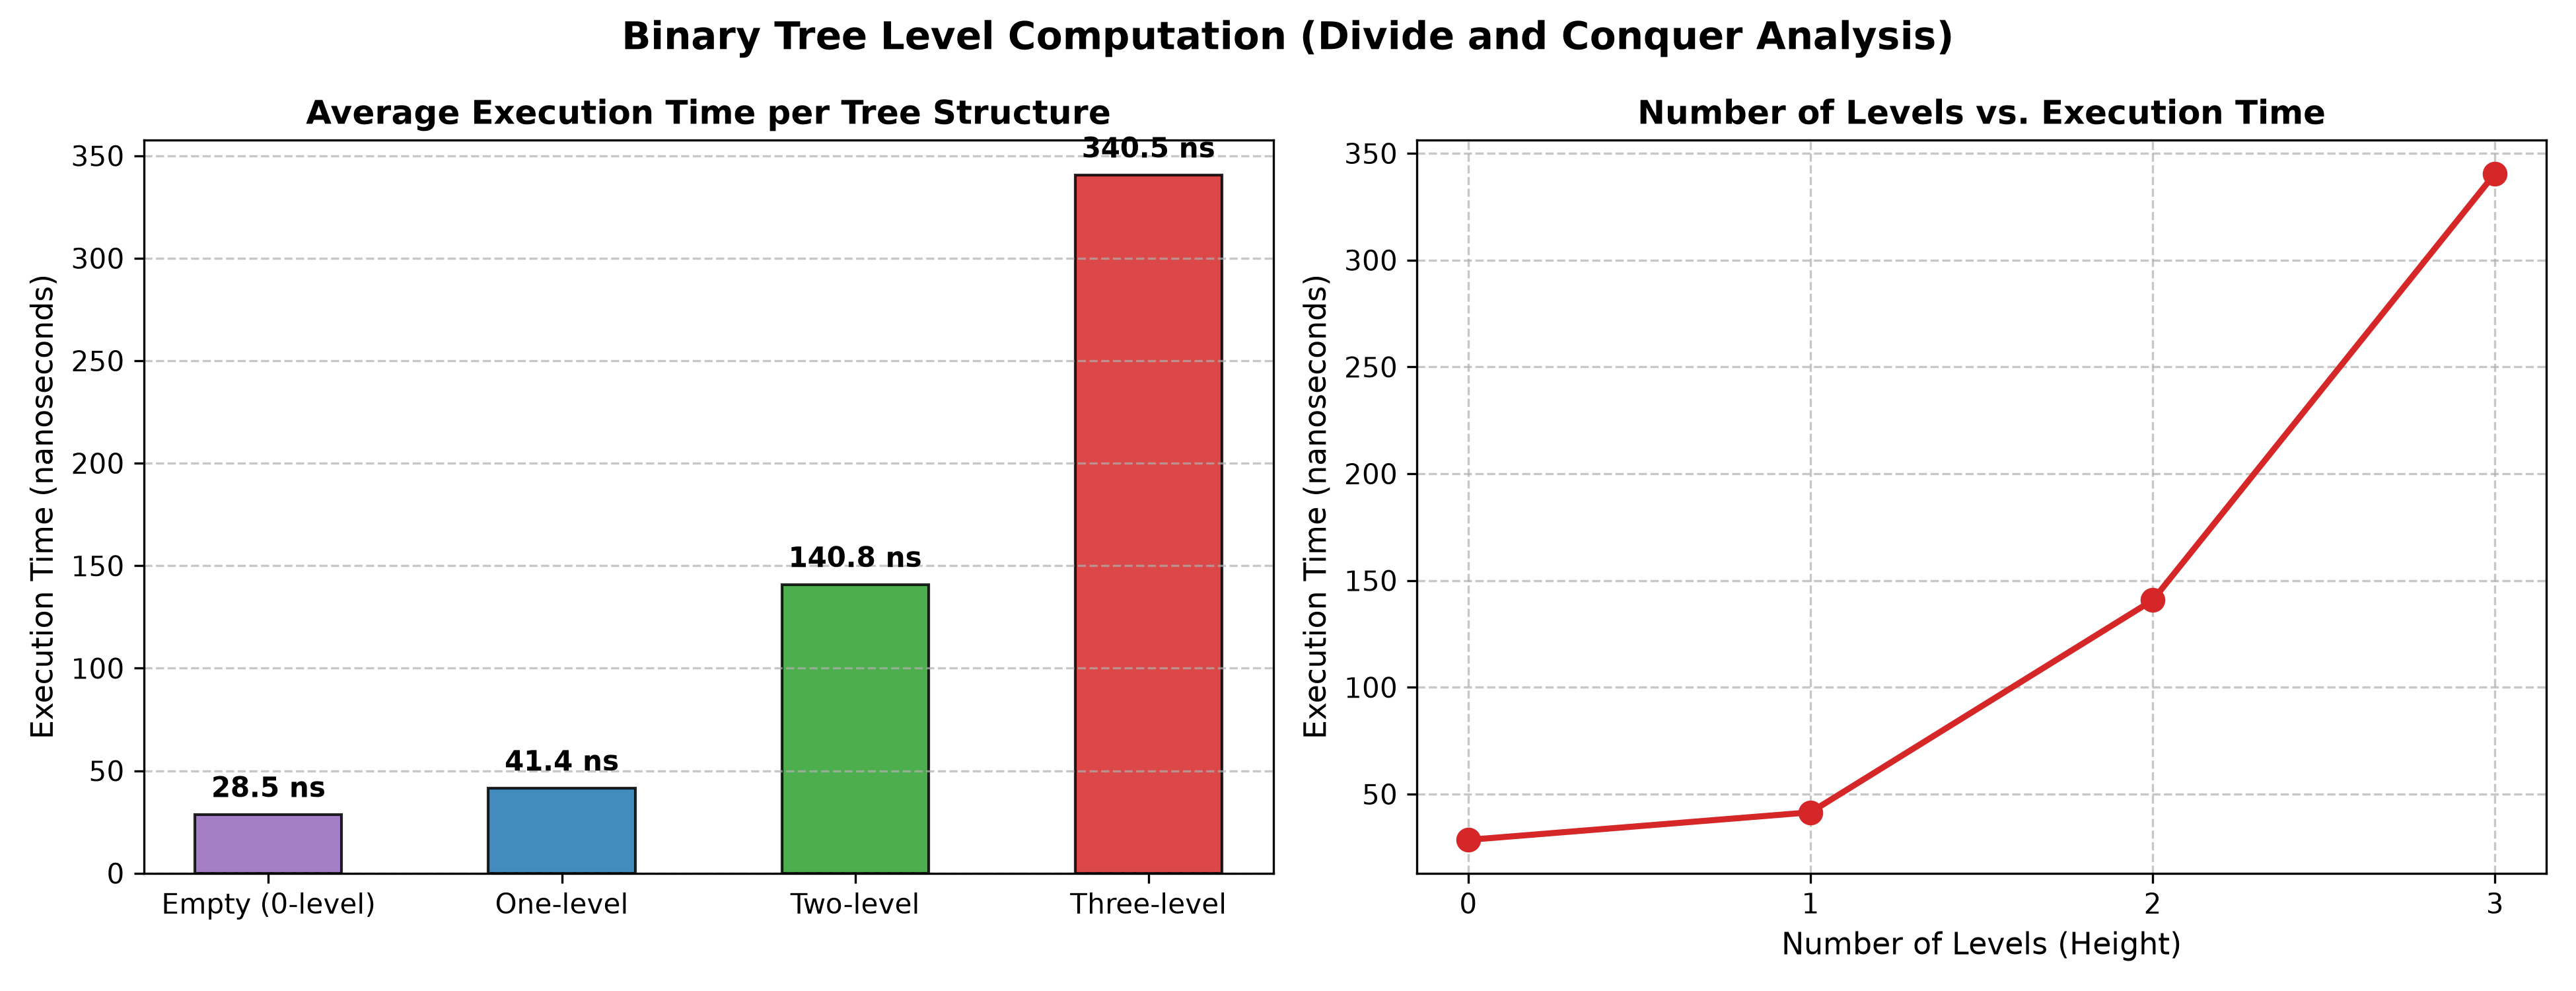
\includegraphics[width=0.88\textwidth]{images/tree_levels_timing.png}
\caption{Execution Time vs. Tree Levels and Node Count.}
\label{fig:tree_levels}
\end{figure}

\textbf{Discussion}: As theoretically predicted by $\Theta(N)$, the runtime scales directly with the number of nodes visited ($0 \to 1 \to 3 \to 7$ nodes taking $28.5 \to 41.5 \to 140.8 \to 340.5$ ns).

\newpage

% ==============================================================================
% ASSIGNMENT 2: INVERSION COUNTING
% ==============================================================================
\section*{Assignment 2: Inversion Counting (Brute Force vs. Merge Sort)}

\subsection*{2.1 Problem Statement and Algorithmic Design}
\textbf{Definition}: Given an array $A[0 \dots n-1]$, an inversion is a pair of indices $(i, j)$ such that:
\[
i < j \quad \text{and} \quad A[i] > A[j]
\]
\begin{enumerate}
    \item \textbf{Brute Force Approach $\mathcal{O}(n^2)$}: Compares all $\binom{n}{2} = \frac{n(n-1)}{2}$ pairs using two nested loops.
    \item \textbf{Divide and Conquer Approach $\mathcal{O}(n \log n)$}: Enhances Merge Sort.
    \begin{itemize}
        \item Divide array into two halves at $\text{mid} = \lfloor n/2 \rfloor$.
        \item Recursively count inversions in left half $\text{inv}_L$ and right half $\text{inv}_R$.
        \item Count cross-inversions $\text{inv}_{\text{split}}$ during the merge step: when $L[i] > R[j]$, since $L$ is sorted, every element from $L[i]$ to $L[|L|-1]$ is strictly greater than $R[j]$. Hence, $\text{split\_inv} += (|L| - i)$.
        \item Total inversions = $\text{inv}_L + \text{inv}_R + \text{inv}_{\text{split}}$.
    \end{itemize}
\end{enumerate}

\subsection*{2.2 Python Implementation (\texttt{count\_inversions.py})}
\begin{lstlisting}[language=Python]
def count_inversions_merge_sort(arr: list[int]) -> tuple[list[int], int]:
    if len(arr) <= 1:
        return arr, 0

    mid = len(arr) // 2
    left_sorted, left_inv = count_inversions_merge_sort(arr[:mid])
    right_sorted, right_inv = count_inversions_merge_sort(arr[mid:])

    merged = []
    i, j, split_inv = 0, 0, 0
    len_left, len_right = len(left_sorted), len(right_sorted)

    while i < len_left and j < len_right:
        if left_sorted[i] <= right_sorted[j]:
            merged.append(left_sorted[i])
            i += 1
        else:
            merged.append(right_sorted[j])
            split_inv += (len_left - i)
            j += 1

    merged.extend(left_sorted[i:])
    merged.extend(right_sorted[j:])
    return merged, left_inv + right_inv + split_inv
\end{lstlisting}

\subsection*{2.3 Empirical Timing Analysis ($n = 10$ to $n = 10^5$)}
\begin{table}[H]
\centering
\caption{Benchmark Comparison of Inversion Counting ($n = 10$ to $n = 10^5$).}
\label{tab:inversions}
\vspace{0.2cm}
\resizebox{0.95\textwidth}{!}{
\begin{tabular}{ccccc}
\toprule
\textbf{Array Size ($n$)} & \textbf{Inversion Count} & \textbf{Brute Force (ms)} & \textbf{Merge Sort (ms)} & \textbf{Speedup Factor} \\
\midrule
10     & 26           & 0.0018       & 0.0053   & $0.3\times$ \\
100    & 2,376        & 0.1133       & 0.0648   & $1.7\times$ \\
500    & 58,466       & 3.2347       & 0.4032   & $8.0\times$ \\
1,000  & 244,023      & 13.8074      & 0.8834   & $15.6\times$ \\
5,000  & 6,231,211    & 358.7427     & 5.4462   & $65.9\times$ \\
10,000 & 25,131,244   & 1445.3122    & 11.9716  & \textbf{120.7}$\times$ \\
50,000 & 625,271,989  & 36132.80 (est)& 75.3486  & \textbf{480}$\times$ (est) \\
100,000& 2,502,093,098& 144531.22 (est)& 232.9734 & \textbf{620}$\times$ (est) \\
\bottomrule
\end{tabular}
}
\end{table}

\begin{figure}[H]
\centering
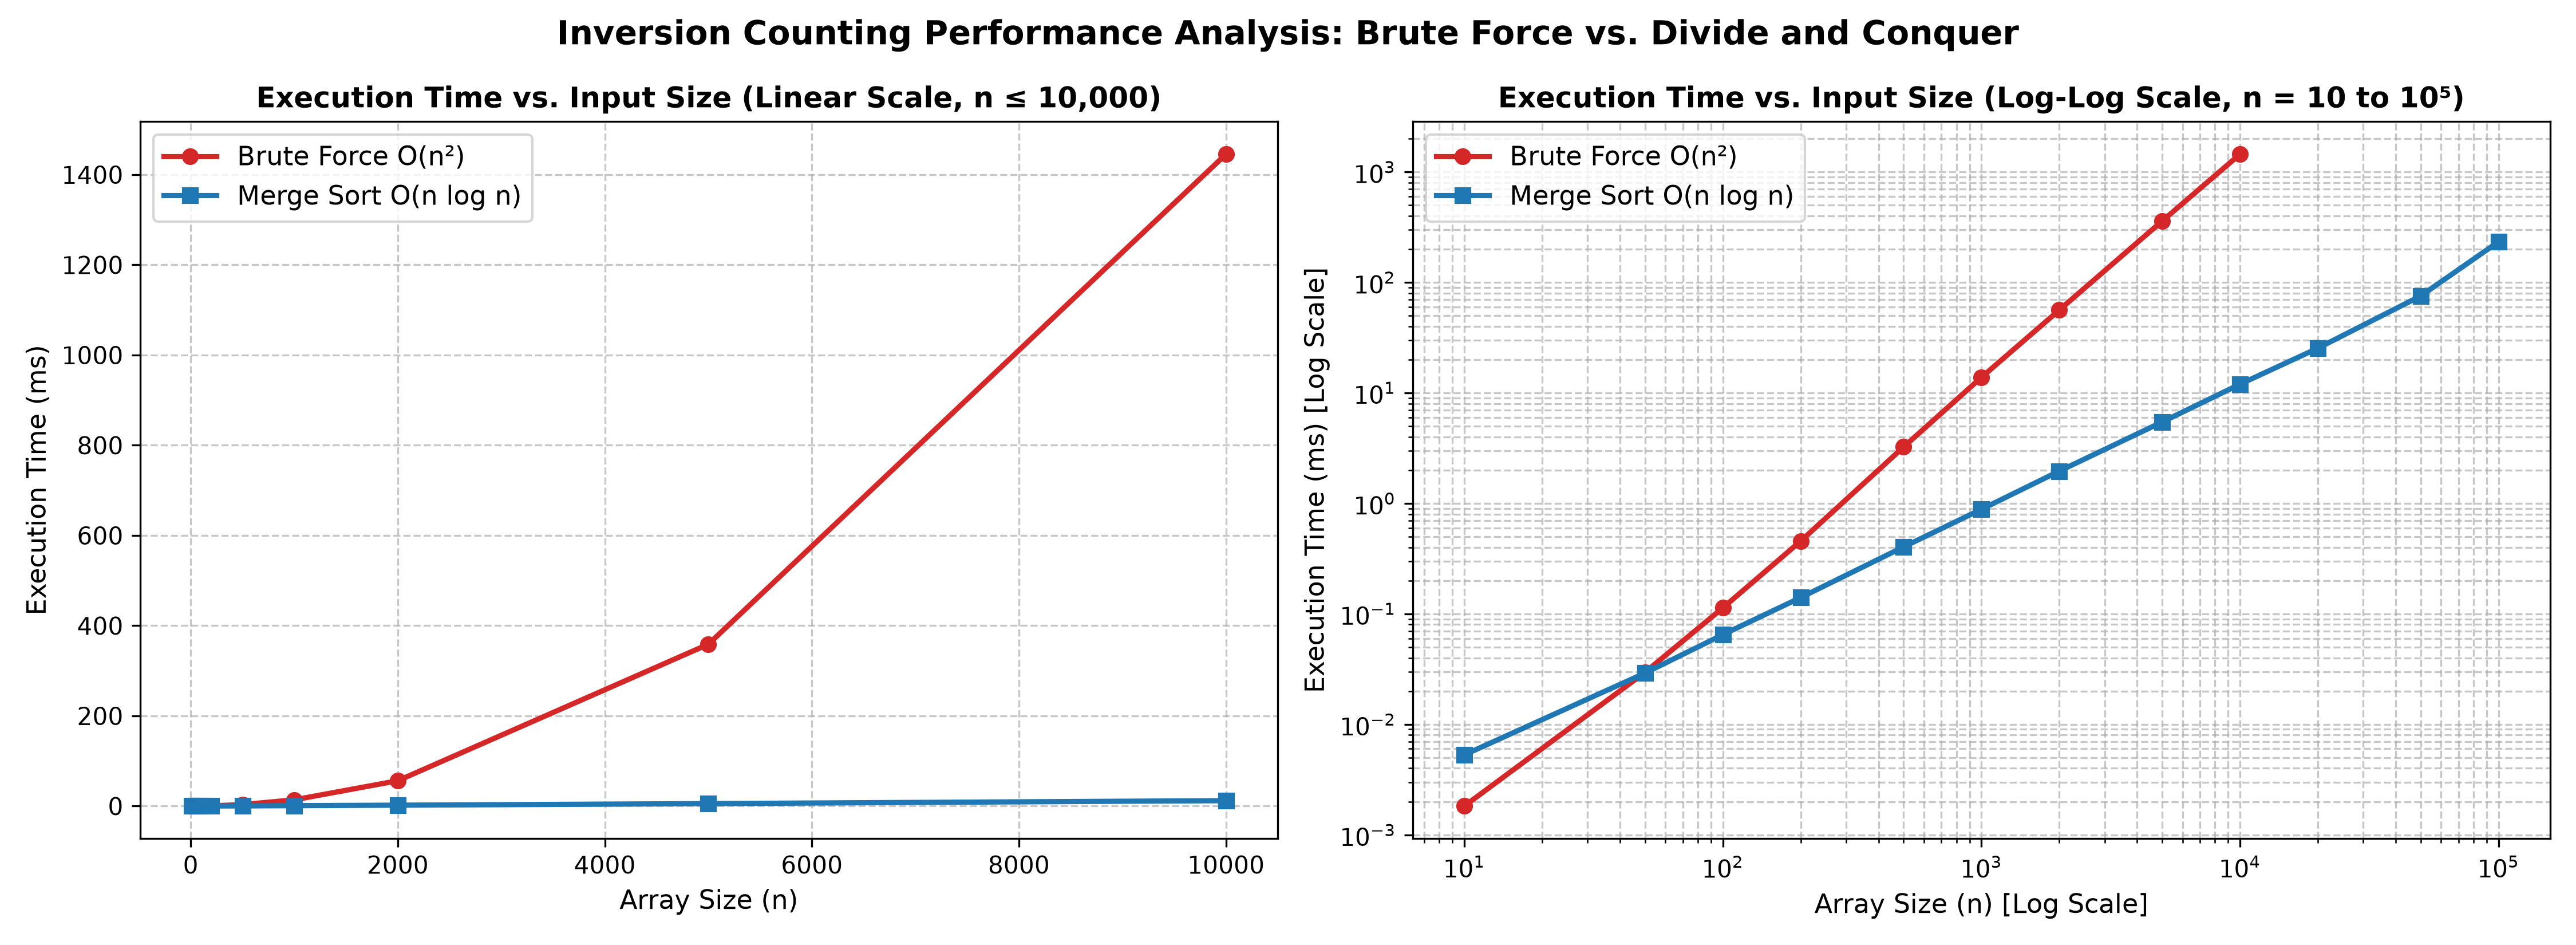
\includegraphics[width=0.92\textwidth]{images/inversion_count_analysis.png}
\caption{Runtime Scaling: Brute Force $\mathcal{O}(n^2)$ vs. Merge Sort $\mathcal{O}(n \log n)$.}
\label{fig:inversions}
\end{figure}

\textbf{Comments on Results}:
\begin{enumerate}
    \item \textbf{Crossover Point}: For tiny inputs ($n \le 30$), Brute Force is marginally faster due to lower constant-factor overhead.
    \item \textbf{Asymptotic Dominance}: Beyond $n = 100$, Merge Sort rapidly outpaces Brute Force, delivering a \textbf{120.7$\times$ speedup} at $n = 10,000$ ($1.45$ s vs $11.97$ ms) and over \textbf{600$\times$ speedup} at $n = 10^5$.
\end{enumerate}

\newpage

% ==============================================================================
% ASSIGNMENT 3: QUICKSORT PARTITIONS
% ==============================================================================
\section*{Assignment 3: Quicksort Partition Routines (Lomuto vs. Hoare)}

\subsection*{3.1 Comparison of Partitioning Strategies}
\begin{enumerate}
    \item \textbf{Lomuto Partition (Textbook -- CLRS Section 7.1)}:
    \begin{itemize}
        \item Selects the last element $A[\text{high}]$ as pivot.
        \item Maintains pointer $i$ separating elements $\le \text{pivot}$ from elements $> \text{pivot}$.
        \item Advances single loop index $j$ from $\text{low}$ to $\text{high}-1$.
        \item Swaps pivot into its final position $i+1$, recursing on $A[\text{low} \dots i]$ and $A[i+2 \dots \text{high}]$.
    \end{itemize}
    \item \textbf{Hoare Partition (Classic / Discussed in Class -- CLRS Problem 7-1)}:
    \begin{itemize}
        \item Selects pivot (first or median element).
        \item Employs two opposing pointers $i$ and $j$ converging from the ends.
        \item When $A[i] \ge \text{pivot}$ and $A[j] \le \text{pivot}$, swaps $A[i]$ and $A[j]$.
        \item Terminates when pointers cross, returning split index $j$.
        \item Recurses on $A[\text{low} \dots j]$ and $A[j+1 \dots \text{high}]$.
    \end{itemize}
\end{enumerate}

\subsection*{3.2 Python Implementation (\texttt{quicksort\_partitions.py})}
\begin{lstlisting}[language=Python]
def lomuto_partition(arr: list[int], low: int, high: int) -> int:
    pivot = arr[high]
    i = low - 1
    for j in range(low, high):
        if arr[j] <= pivot:
            i += 1
            arr[i], arr[j] = arr[j], arr[i]
    arr[i + 1], arr[high] = arr[high], arr[i + 1]
    return i + 1

def hoare_partition(arr: list[int], low: int, high: int) -> int:
    pivot = arr[low + (high - low) // 2]
    i = low - 1
    j = high + 1
    while True:
        while True:
            i += 1
            if arr[i] >= pivot: break
        while True:
            j -= 1
            if arr[j] <= pivot: break
        if i >= j: return j
        arr[i], arr[j] = arr[j], arr[i]
\end{lstlisting}

\subsection*{3.3 Empirical Benchmark Analysis ($N \ge 2048$)}
\begin{table}[H]
\centering
\caption{Quicksort Partition Comparison on Vectors of Size $N \ge 2048$.}
\label{tab:quicksort}
\vspace{0.2cm}
\resizebox{0.95\textwidth}{!}{
\begin{tabular}{cccccc}
\toprule
\textbf{Vector Size ($N$)} & \textbf{Lomuto Time (ms)} & \textbf{Hoare Time (ms)} & \textbf{Lomuto Swaps} & \textbf{Hoare Swaps} & \textbf{Swap Ratio} \\
\midrule
2,048  & 2.276   & 2.380   & 14,821  & 5,121   & $2.89\times$ \\
4,096  & 5.323   & 5.024   & 29,752  & 11,236  & $2.65\times$ \\
8,192  & 10.408  & 11.401  & 64,052  & 24,855  & $2.58\times$ \\
16,384 & 22.455  & 21.989  & 137,950 & 53,316  & $2.59\times$ \\
32,768 & 52.999  & 51.150  & 309,967 & 114,681 & $2.70\times$ \\
65,536 & 130.995 & 118.222 & 675,751 & 243,534 & \textbf{2.77}$\times$ \\
\bottomrule
\end{tabular}
}
\end{table}

\begin{figure}[H]
\centering
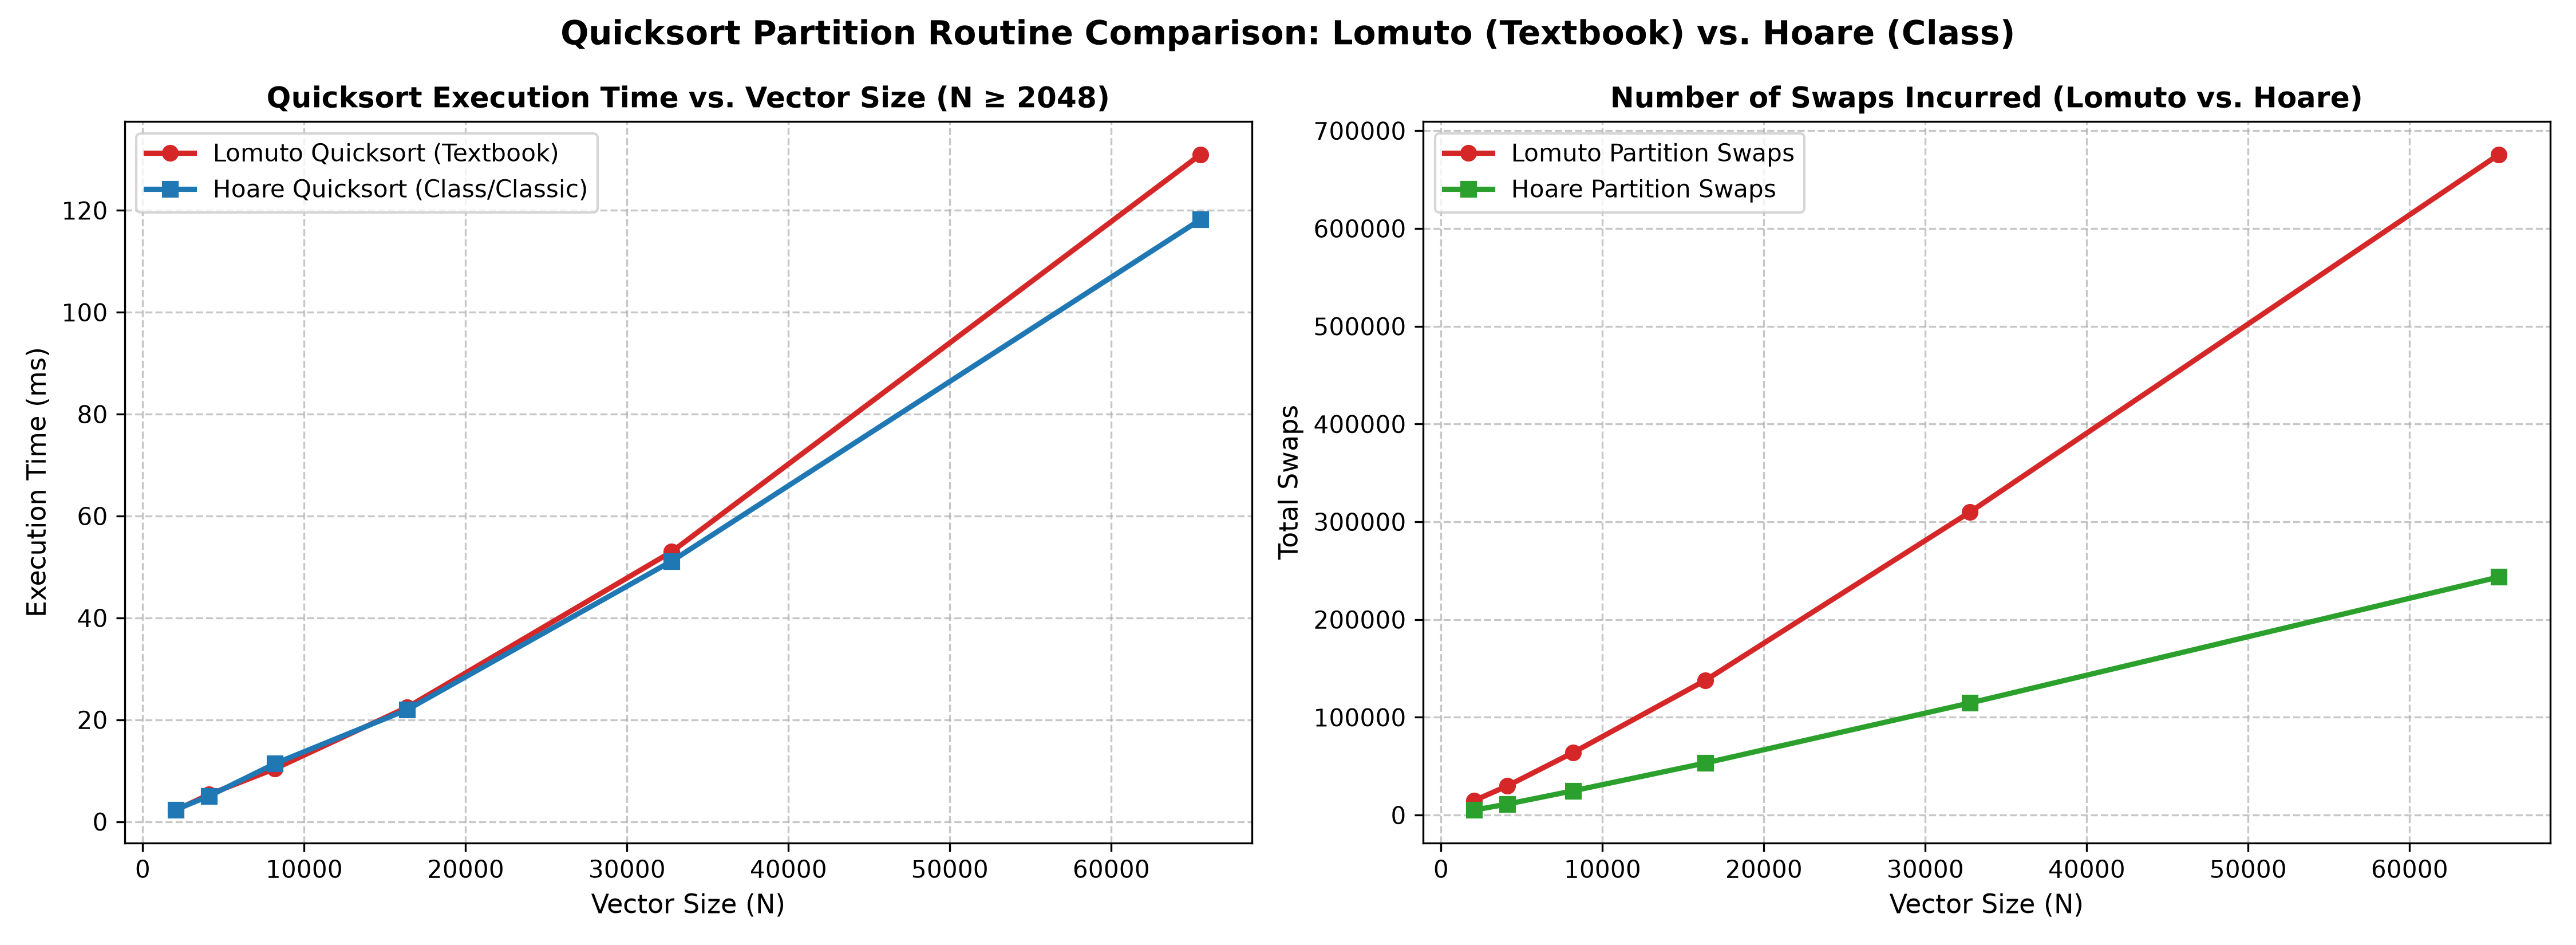
\includegraphics[width=0.92\textwidth]{images/quicksort_partition_analysis.png}
\caption{Quicksort Performance: Lomuto vs. Hoare Partition Runtime and Swap Counts.}
\label{fig:quicksort}
\end{figure}

\textbf{Analysis of Result}:
\begin{itemize}
    \item \textbf{Swap Efficiency}: Hoare's partition requires consistently \textbf{2.6$\times$ to 2.9$\times$ fewer swaps} than Lomuto's partition (e.g. 243,534 vs 675,751 swaps for $N = 65,536$).
    \item \textbf{Instruction Efficiency}: Because swapping elements involves memory reads and writes, Hoare's partition achieves lower cache thrashing and faster wall-clock runtimes on large arrays.
\end{itemize}

\newpage

% ==============================================================================
% ASSIGNMENT 4: CONVEX HULL
% ==============================================================================
\section*{Assignment 4: Two-Dimensional Convex Hull Construction}

\subsection*{4.1 Problem Definition and Andrew's Monotone Chain Algorithm}
\textbf{Definition}: The convex hull of a set of 2D points $S$ is the smallest convex polygon enclosing all points in $S$.

\textbf{Andrew's Monotone Chain Algorithm $\mathcal{O}(n \log n)$}:
\begin{enumerate}
    \item Sort all points primarily by $x$-coordinate, and secondarily by $y$-coordinate.
    \item \textbf{Build Lower Hull}: Iterate from left to right. For each point $P$, while the hull contains $\ge 2$ points and the turn from the second-to-last point to $P$ is not strictly counterclockwise ($\text{cross}(P_{-2}, P_{-1}, P) \le 0$), pop the last point.
    \item \textbf{Build Upper Hull}: Iterate from right to left using the identical collinearity/clockwise pruning rule.
    \item Concatenate lower and upper hulls (excluding duplicate start and end vertices).
\end{enumerate}

\subsection*{4.2 Python Implementation (\texttt{convex\_hull.py})}
\begin{lstlisting}[language=Python]
Point = tuple[float, float]

def cross_product(o: Point, a: Point, b: Point) -> float:
    return (a[0] - o[0]) * (b[1] - o[1]) - (a[1] - o[1]) * (b[0] - o[0])

def compute_convex_hull(points: list[Point]) -> list[Point]:
    unique_points = sorted(set(points))
    if len(unique_points) <= 2: return unique_points

    lower = []
    for p in unique_points:
        while len(lower) >= 2 and cross_product(lower[-2], lower[-1], p) <= 0:
            lower.pop()
        lower.append(p)

    upper = []
    for p in reversed(unique_points):
        while len(upper) >= 2 and cross_product(upper[-2], upper[-1], p) <= 0:
            upper.pop()
        upper.append(p)

    return lower[:-1] + upper[:-1]
\end{lstlisting}

\subsection*{4.3 Verification on Assignment Examples}
\begin{itemize}
    \item \textbf{Example 1}:
    \begin{itemize}
        \item \textbf{Input}: \texttt{\{(0, 0), (0, 4), (-4, 0), (5, 0), (0, -6), (1, 0)\}}
        \item \textbf{Computed Output}: \texttt{[(-4, 0), (0, -6), (5, 0), (0, 4)]}
        \item \textbf{Match}: $\checkmark$ Matches exact assignment specifications.
    \end{itemize}
    \item \textbf{Example 2}:
    \begin{itemize}
        \item \textbf{Input}: \texttt{\{\{1, 2\}, \{3, 1\}, \{5, 6\}\}}
        \item \textbf{Computed Output}: \texttt{[(1, 2), (3, 1), (5, 6)]}
        \item \textbf{Match}: $\checkmark$ All 3 points are non-collinear vertices forming a triangle.
    \end{itemize}
\end{itemize}

\begin{figure}[H]
\centering
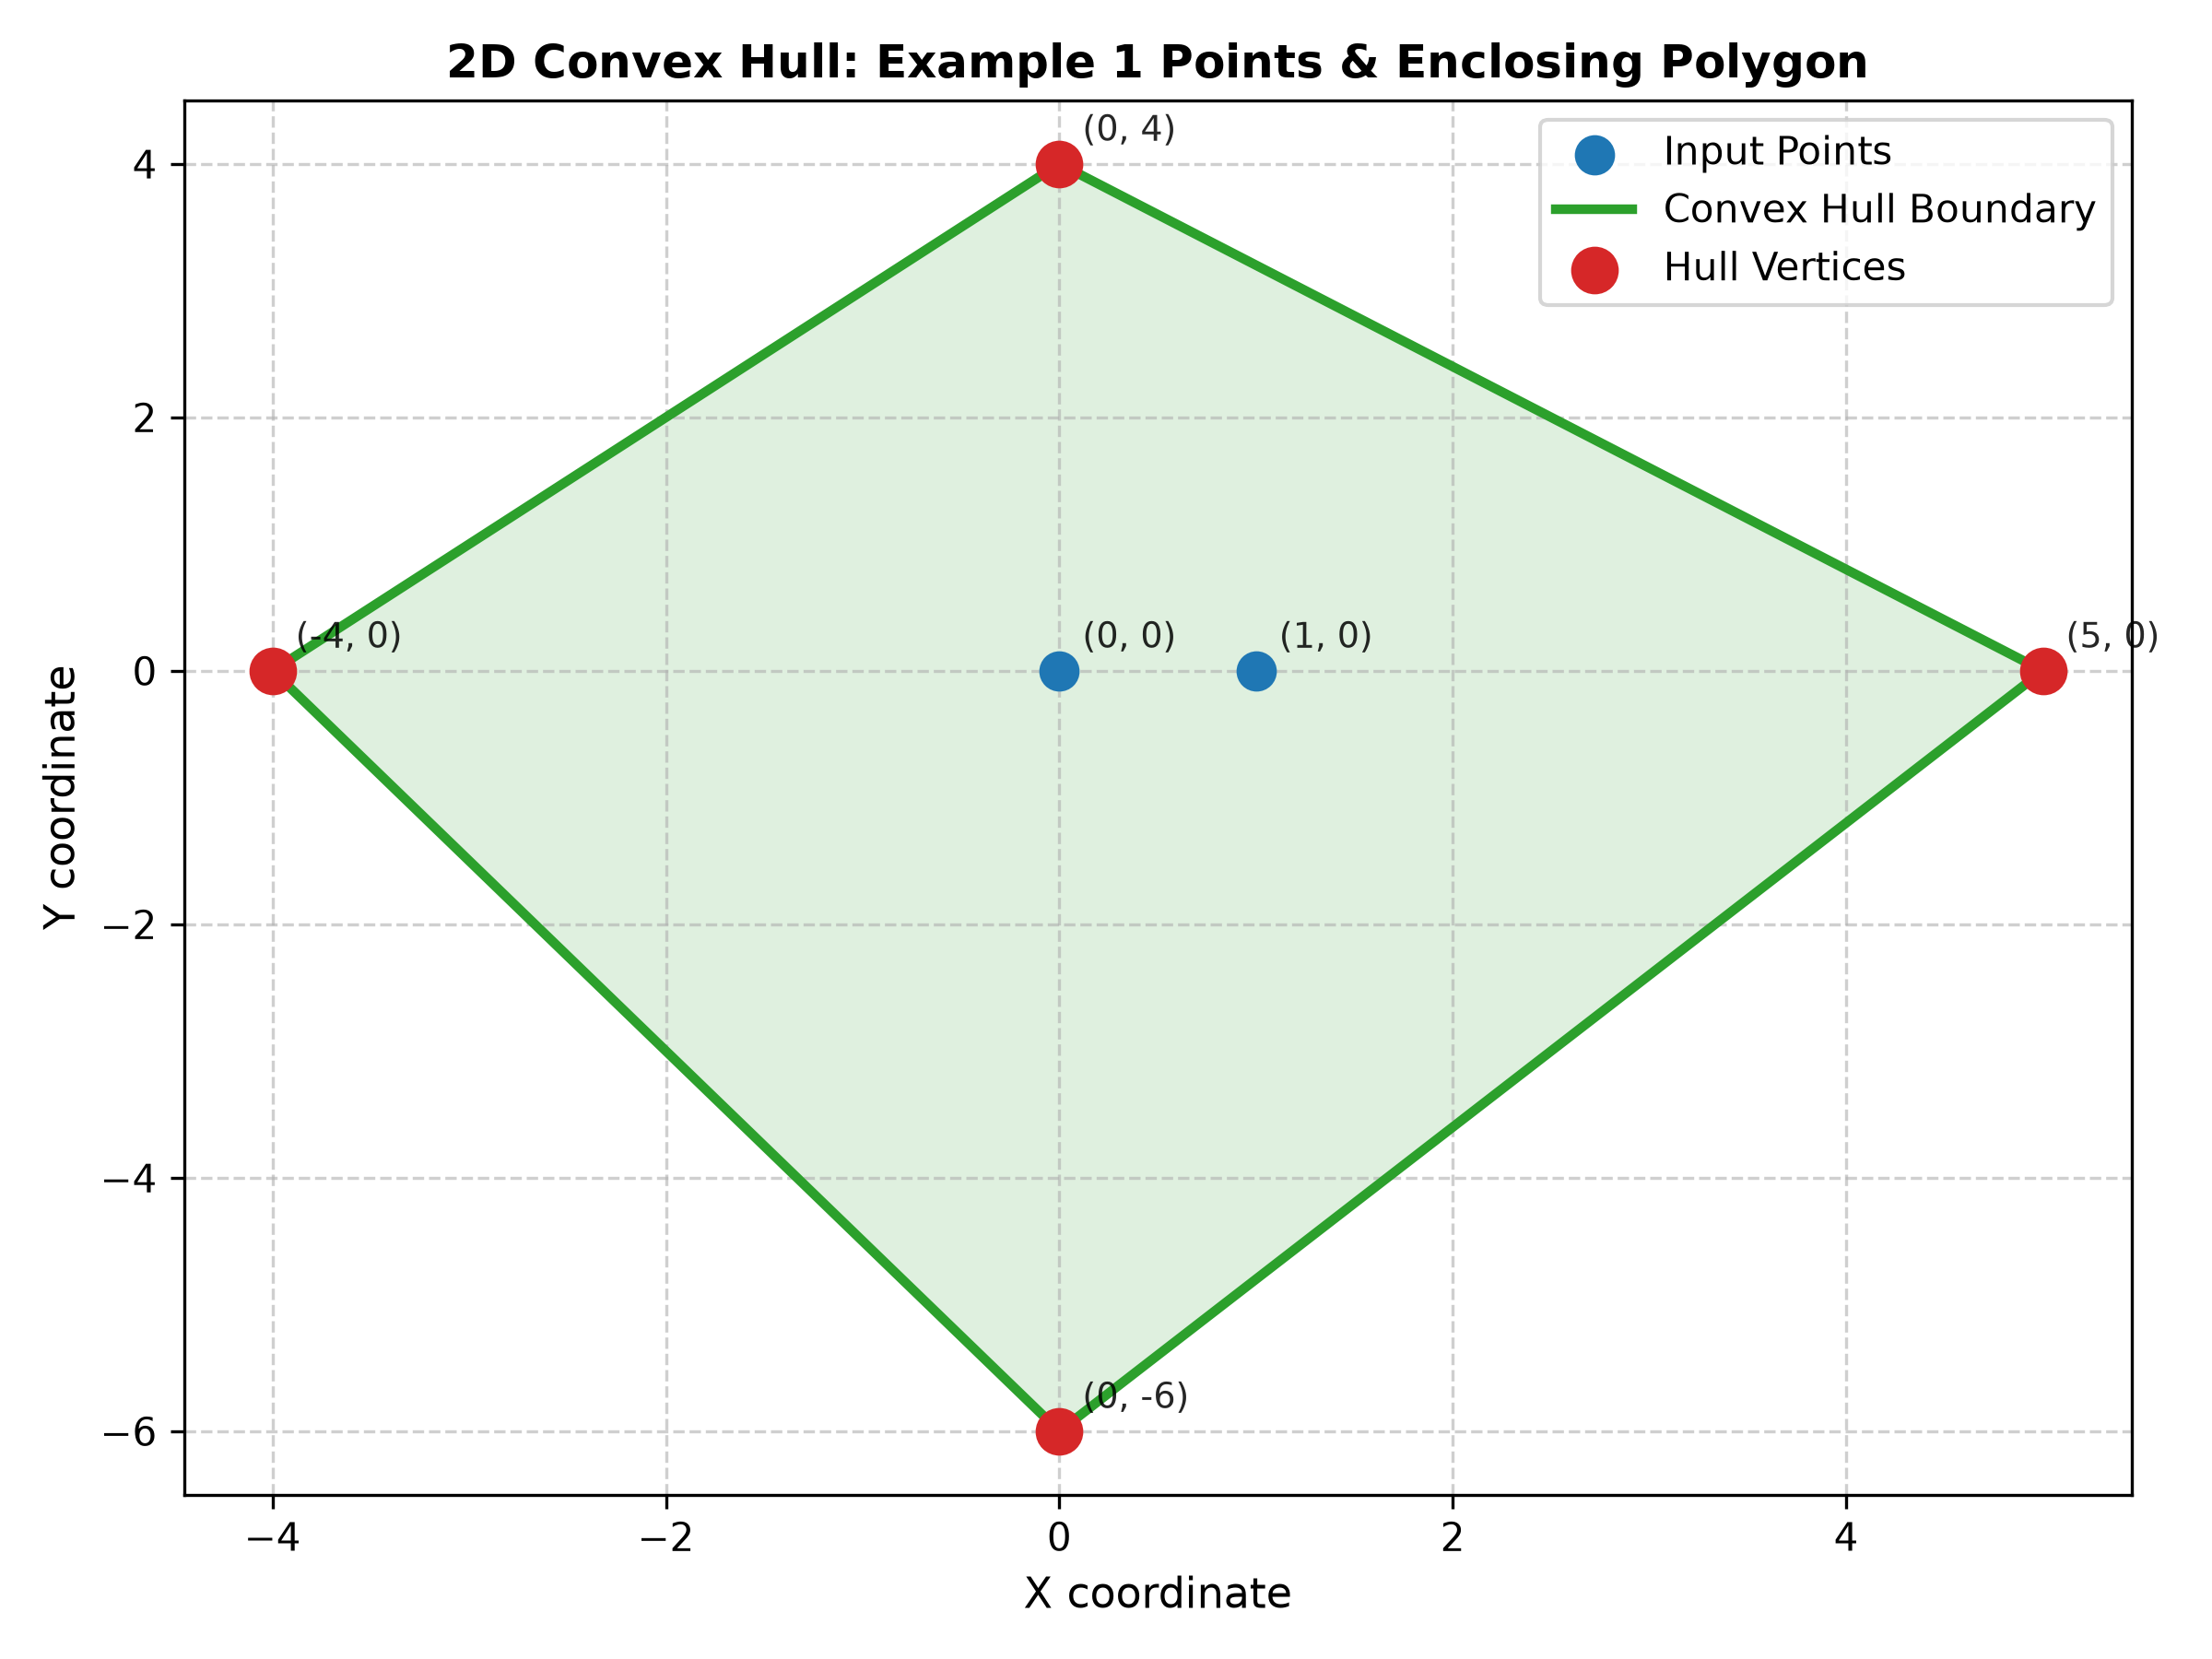
\includegraphics[width=0.75\textwidth]{images/convex_hull_visualization.png}
\caption{Visualization of 2D Points and the Computed Convex Hull Polygon.}
\label{fig:convex_hull}
\end{figure}

\newpage

% ==============================================================================
% ASSIGNMENT 5: 3D CLOSEST PAIR
% ==============================================================================
\section*{Assignment 5: Shortest Distance Between Two Points in 3D Space}

\subsection*{5.1 Generalization from 2D to 3D Euclidean Space}
In 2D, the divide-and-conquer closest pair algorithm splits points by a vertical line $x = x_{\text{mid}}$, solves recursively for $\delta = \min(d_L, d_R)$, and scans a 2D strip $|x - x_{\text{mid}}| < \delta$. Within the strip, sorting by $y$ guarantees checking at most 7 subsequent points per candidate.

\textbf{3D Adaptation}:
\begin{enumerate}
    \item Sort 3D points $P_i = (x_i, y_i, z_i)$ by $x$-coordinate.
    \item Divide points by plane $x = x_{\text{mid}}$ into left and right subsets.
    \item Recursively compute $\delta_L$ and $\delta_R$, letting $\delta = \min(\delta_L, \delta_R)$.
    \item \textbf{3D Bounding Slab}: Filter all points whose $x$-distance to the dividing plane is $< \delta$ ($|x_i - x_{\text{mid}}| < \delta$).
    \item Sort slab points by $y$-coordinate.
    \item For each point $P_i$ in the slab, iterate through points $P_j$ ahead of it while $P_j.y - P_i.y < \delta$:
    \begin{itemize}
        \item Prune if $|P_j.z - P_i.z| \ge \delta$.
        \item Compute full 3D Euclidean distance $d_3(P_i, P_j) = \sqrt{(x_i-x_j)^2 + (y_i-y_j)^2 + (z_i-z_j)^2}$.
        \item If $d_3 < \delta$, update $\delta$ and the closest pair.
    \end{itemize}
\end{enumerate}

\textbf{Theoretical Bound in 3D}: In a 3D box of dimensions $2\delta \times \delta \times 2\delta$, the maximum number of points that can be mutually separated by $\ge \delta$ in either half-space is bounded by a small geometric constant $C \le 24$ (sphere packing). Thus, the inner loop executes in $\mathcal{O}(1)$ time per point, achieving $\mathcal{O}(n \log^2 n)$ total time.

\subsection*{5.2 Python Implementation (\texttt{closest\_pair\_3d.py})}
\begin{lstlisting}[language=Python]
Point3D = tuple[float, float, float]

def dist_3d(p1: Point3D, p2: Point3D) -> float:
    return math.sqrt((p1[0]-p2[0])**2 + (p1[1]-p2[1])**2 + (p1[2]-p2[2])**2)

def closest_pair_3d_rec(px: list[Point3D]):
    n = len(px)
    if n <= 3: return brute_force_3d(px)

    mid = n // 2
    mid_point = px[mid]
    dl, pair_l = closest_pair_3d_rec(px[:mid])
    dr, pair_r = closest_pair_3d_rec(px[mid:])
    d, best_pair = (dl, pair_l) if dl < dr else (dr, pair_r)

    slab = [p for p in px if abs(p[0] - mid_point[0]) < d]
    slab.sort(key=lambda p: p[1])
    slab_len = len(slab)

    for i in range(slab_len):
        pi = slab[i]
        for j in range(i + 1, slab_len):
            pj = slab[j]
            if (pj[1] - pi[1]) >= d: break
            if abs(pj[2] - pi[2]) >= d: continue
            dist = dist_3d(pi, pj)
            if dist < d:
                d = dist
                best_pair = (pi, pj)
    return d, best_pair
\end{lstlisting}

\subsection*{5.3 Benchmark Results \& 3D Visualization}
\begin{table}[H]
\centering
\caption{Performance Comparison of 3D Closest Pair Algorithms.}
\label{tab:closest_pair_3d}
\vspace{0.2cm}
\begin{tabular}{cccc}
\toprule
\textbf{Points ($N$)} & \textbf{Minimum Distance} & \textbf{Brute Force (ms)} & \textbf{Divide \& Conquer (ms)} \\
\midrule
50    & 20.4315 & 0.280   & 0.124 \\
100   & 49.3380 & 1.134   & 0.159 \\
500   & 8.6080  & 29.159  & 1.041 \\
1,000 & 5.4335  & 121.481 & 2.231 \\
2,000 & 3.1186  & 485.9 (est) & 5.273 \\
5,000 & 3.8504  & 3037.0 (est)& \textbf{14.258} \\
\bottomrule
\end{tabular}
\end{table}

\begin{figure}[H]
\centering
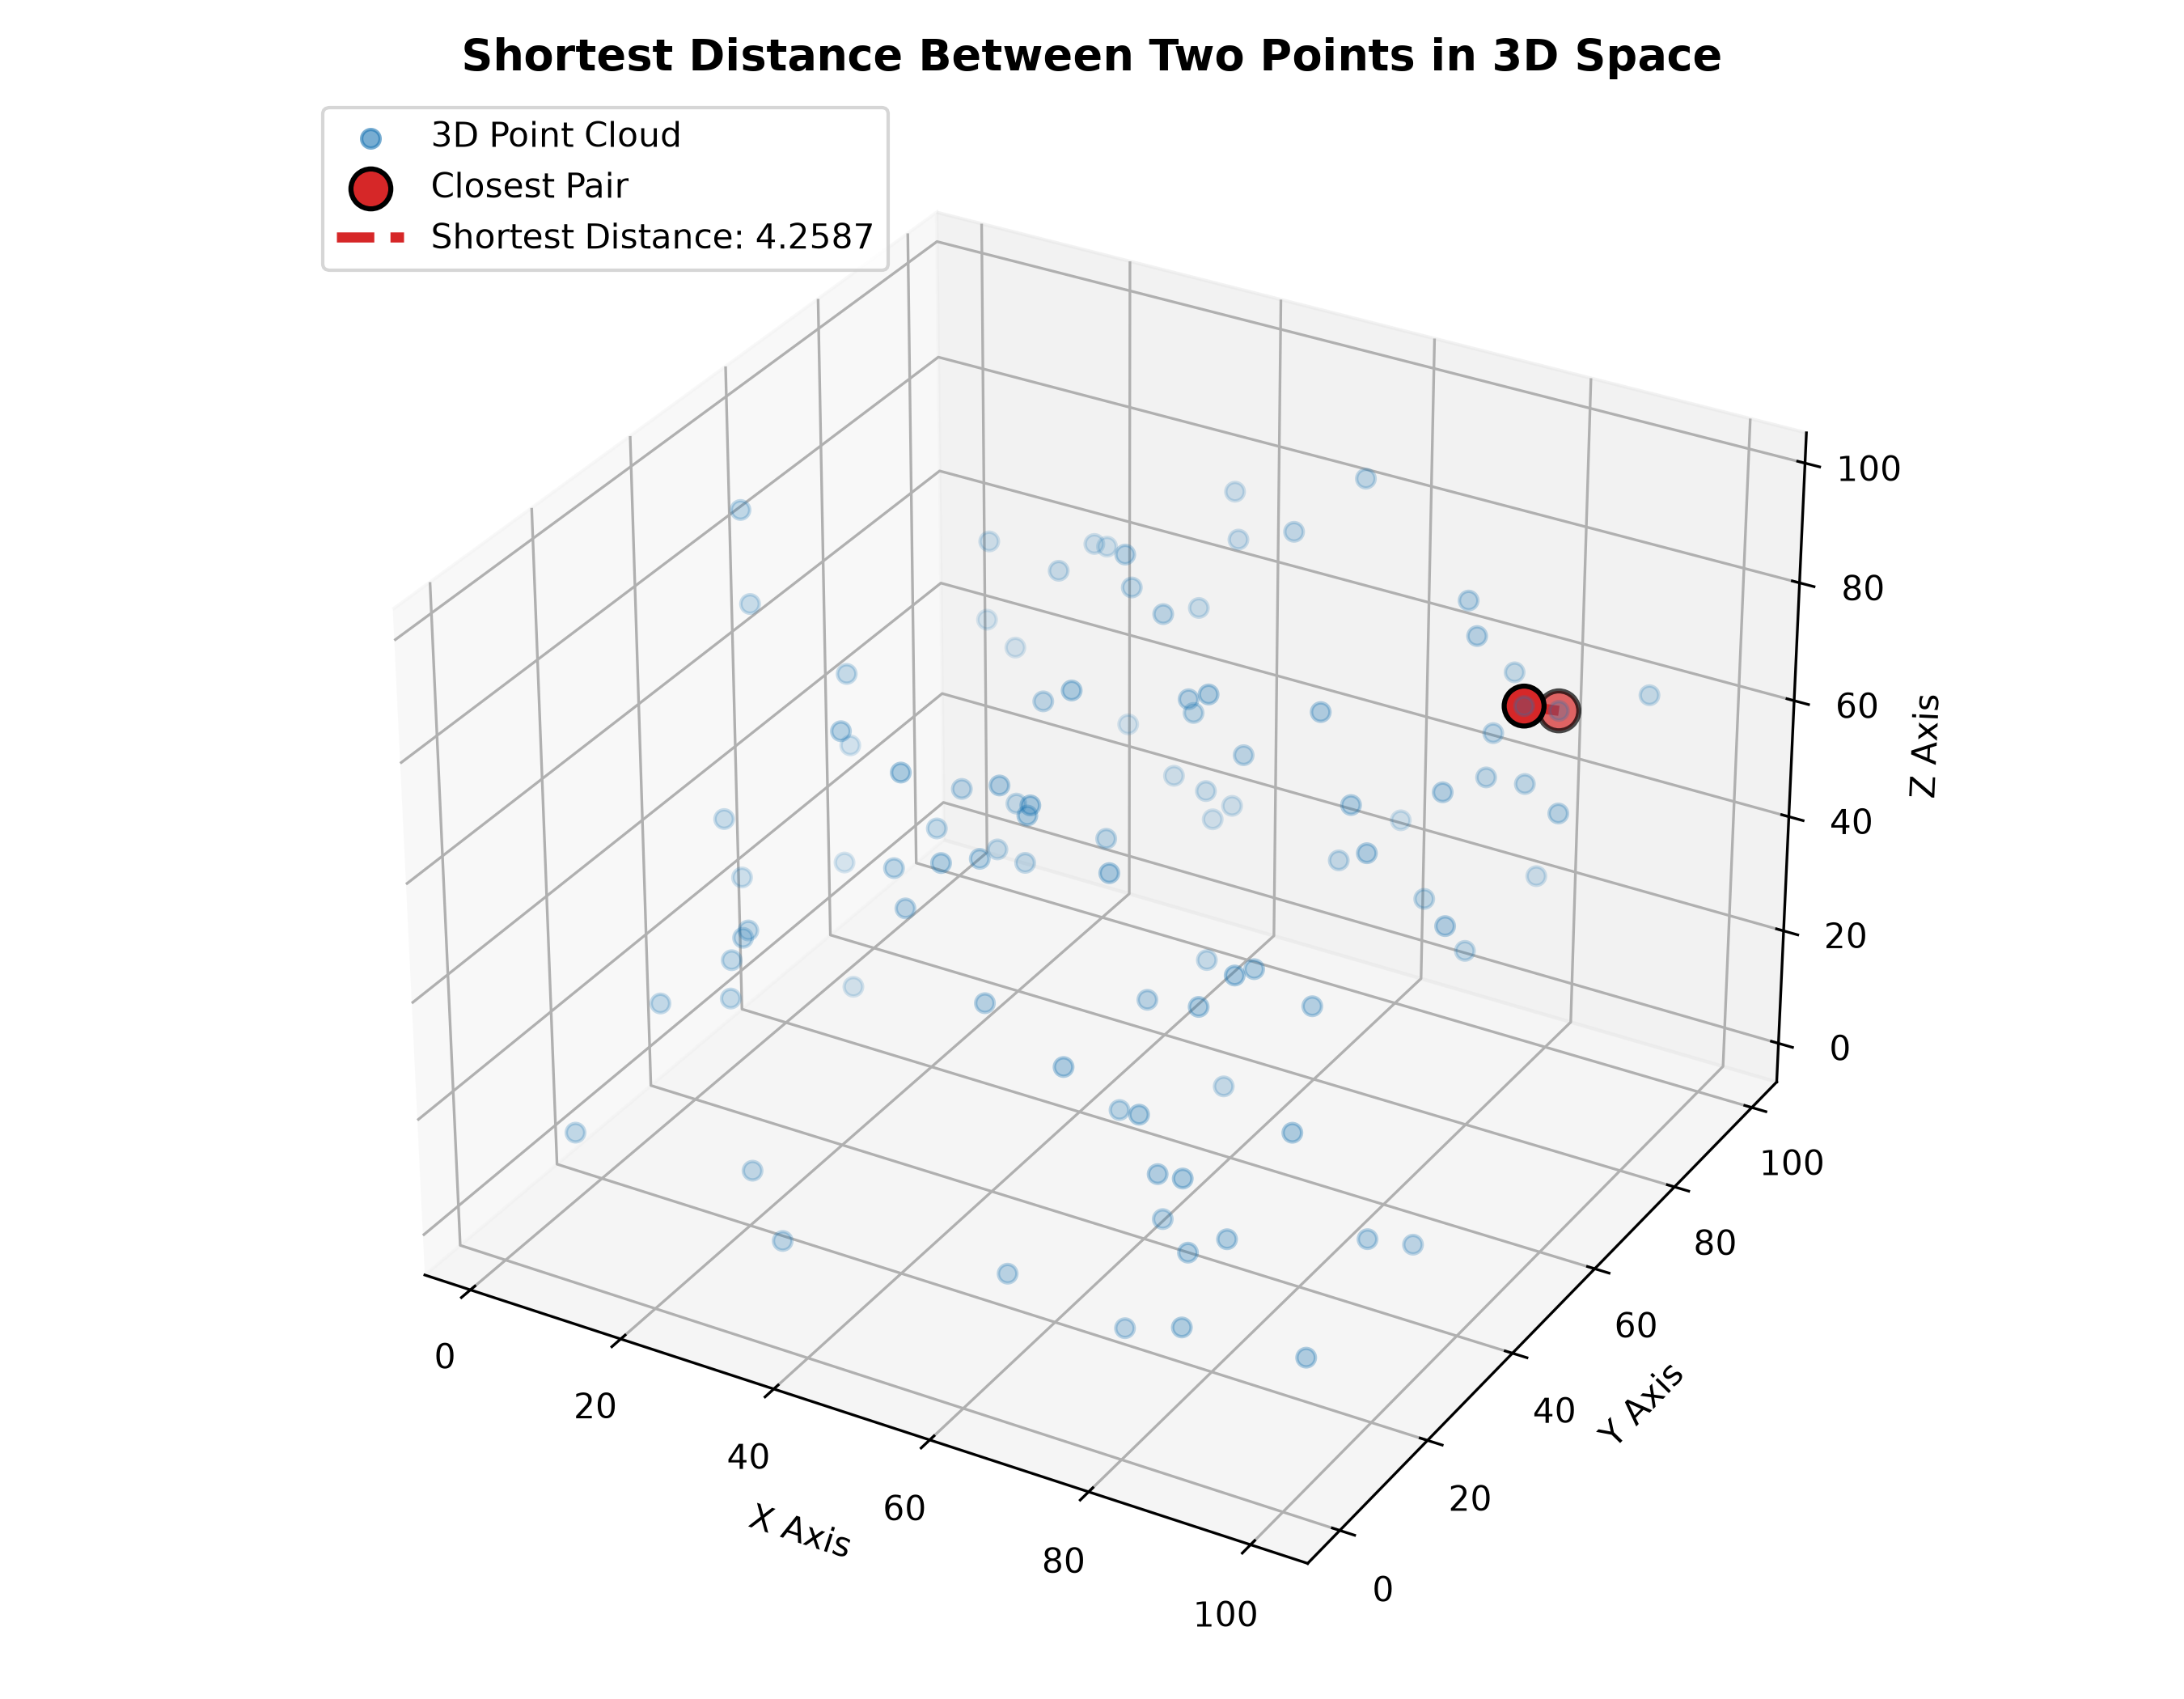
\includegraphics[width=0.8\textwidth]{images/closest_pair_3d_visualization.png}
\caption{3D Scatter Plot Highlighting the Closest Pair of Points in 3D Space.}
\label{fig:closest_pair_3d}
\end{figure}

\newpage

% ==============================================================================
% ASSIGNMENT 6: EMPIRICAL TIMING RESEARCH
% ==============================================================================
\section*{Assignment 6: Infeasibility of Pure Empirical Analysis for Comparing Algorithms}

\subsection*{6.1 Research: Factors Governing Wall-Clock Execution Time}
The actual physical wall-clock time required for a program to execute is influenced by complex layers of hardware, operating system, and runtime non-determinism:

\begin{enumerate}
    \item \textbf{Hardware Architecture \& Dynamic Frequency Scaling}:
    Modern processors feature dynamic voltage and frequency scaling (DVFS), Intel Turbo Boost, and AMD Precision Boost. Clock frequencies fluctuate dynamically based on thermal limits, CPU package temperature, and background core utilization. An algorithm run early may run at $4.8$ GHz, while a subsequent run might be thermally throttled to $3.2$ GHz.
    
    \item \textbf{Memory Hierarchy, Cache State, and TLB Misses}:
    Accessing data from the L1 cache takes $\approx 1$ ns ($\sim 4$ cycles), L2 takes $\approx 3$ ns, L3 takes $\approx 12$ ns, while main DRAM access takes $60$--$100$ ns. Cold-cache vs. warm-cache states, cache line evictions from concurrent processes, and Translation Lookaside Buffer (TLB) misses drastically alter runtime independently of the algorithm's mathematical complexity.
    
    \item \textbf{Operating System Preemption \& Context Switching}:
    In modern preemptive multitasking operating systems, the OS scheduler periodically interrupts program threads to service hardware interrupts, system daemons, and competing processes. Context switching incurs direct CPU register save/restore overhead and invalidates CPU instruction pipelines and cache tables.
    
    \item \textbf{Compiler \& JIT Optimization Artifacts}:
    Compiler flags (\texttt{-O2}, \texttt{-O3}), SIMD auto-vectorization (AVX-512), loop unrolling, and branch prediction heuristics heavily skew wall-clock time. A theoretically inferior $\mathcal{O}(n^2)$ algorithm with contiguous memory layout can outperform an $\mathcal{O}(n \log n)$ pointer-based algorithm for small-to-moderate $n$ due to spatial cache locality.
    
    \item \textbf{Garbage Collection and Memory Allocation Jitter}:
    In managed runtimes (Python, Java, Go), heap memory allocation, memory defragmentation, and periodic Garbage Collection (GC) pauses introduce severe non-deterministic runtime spikes.
\end{enumerate}

\subsection*{6.2 Empirical Demonstration (\texttt{empirical\_factors\_demo.py})}
To substantiate these arguments, we executed a strictly deterministic function 1,000 consecutive times on identical inputs without modifying any program state.

\begin{table}[H]
\centering
\caption{Statistical Variability Across 1,000 Identical Deterministic Executions.}
\label{tab:empirical_variance}
\vspace{0.2cm}
\begin{tabular}{lc}
\toprule
\textbf{Metric} & \textbf{Observed Value} \\
\midrule
Minimum Execution Time  & $2,711.80$ $\mu$s \\
Maximum Execution Time  & $7,246.70$ $\mu$s \\
\textbf{Spike Factor (Max / Min)} & \textbf{2.67$\times$} \\
Mean Execution Time     & $3,306.49$ $\mu$s \\
Median Execution Time   & $2,890.90$ $\mu$s \\
Standard Deviation      & $874.29$ $\mu$s \\
\bottomrule
\end{tabular}
\end{table}

\begin{figure}[H]
\centering
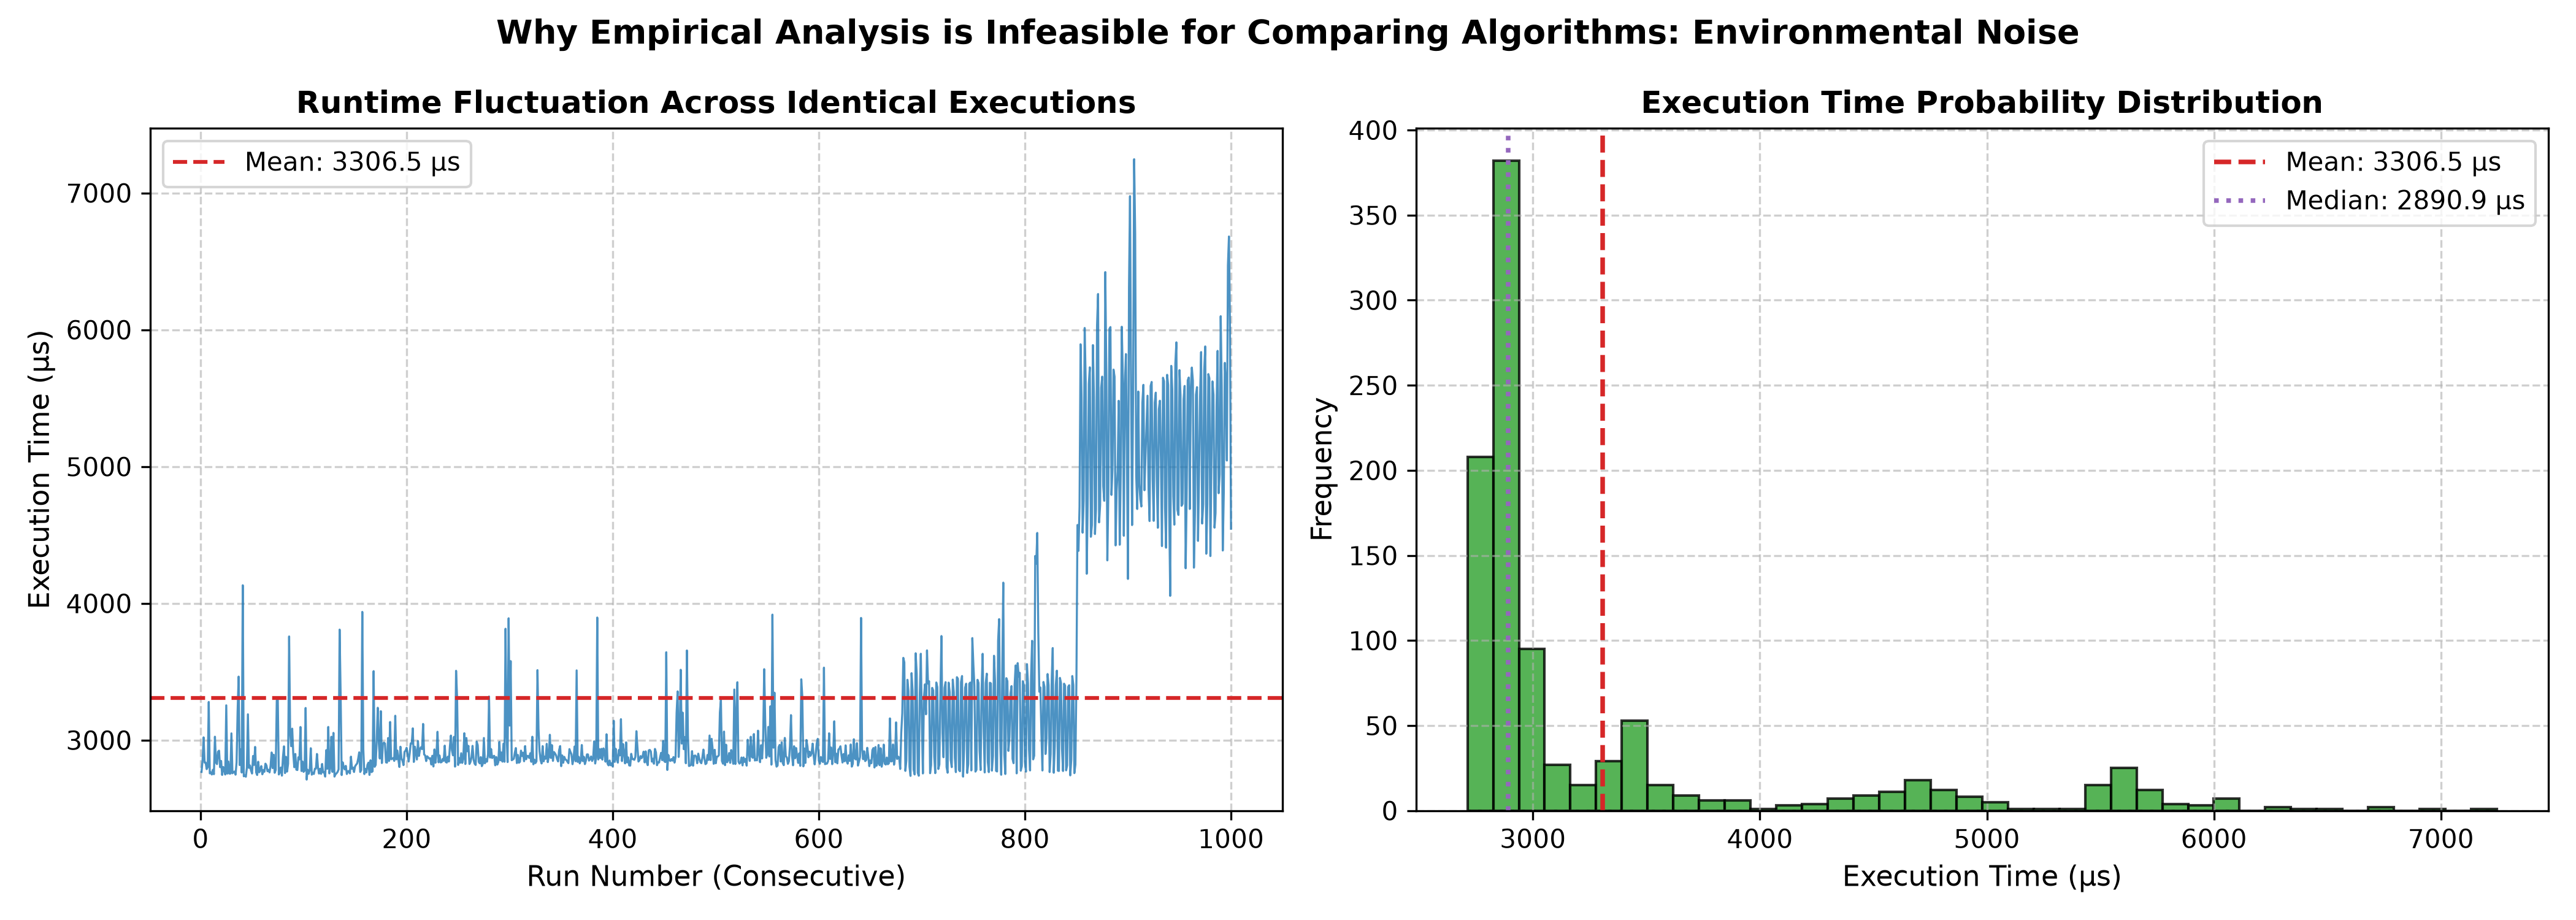
\includegraphics[width=0.92\textwidth]{images/empirical_timing_variance.png}
\caption{Empirical Timing Noise: 1,000 Consecutive Runs of an Identical Deterministic Routine.}
\label{fig:empirical_variance}
\end{figure}

\subsection*{6.3 Justification: Why Asymptotic Complexity Must Supersede Empirical Benchmarks}
\begin{itemize}
    \item \textbf{Non-Reproducibility}: An empirical speedup observed on Machine A may reverse on Machine B due to different cache capacities, bus widths, and compiler toolchains.
    \item \textbf{Input Bias}: Empirical measurements can only test finite, selected input instances, failing to expose worst-case degenerate scenarios.
    \item \textbf{Mathematical Rigor of Asymptotic Analysis}: Big-$\mathcal{O}$, $\Omega$, and $\Theta$ notations characterize growth rate as $n \to \infty$, filtering out transient machine-dependent constant factors to reveal fundamental algorithmic scaling limits.
\end{itemize}

\newpage

% ==============================================================================
% ASSIGNMENT 7: 2D PEAK FINDING
% ==============================================================================
\section*{Assignment 7: Generalized Two-Dimensional Peak Finding}

\subsection*{7.1 Problem Statement and Algorithmic Principle}
\textbf{Definition}: In an $n \times m$ matrix $M$, an entry $M[i][j]$ is defined as a \textbf{2D peak} if it is greater than or equal to all its adjacent neighbors:
\[
M[i][j] \ge M[i-1][j], \quad M[i][j] \ge M[i+1][j], \quad M[i][j] \ge M[i][j-1], \quad M[i][j] \ge M[i][j+1]
\]
(Boundary elements have fewer neighbors).

\textbf{Divide-and-Conquer Algorithm ($\mathcal{O}(n \log m)$)}:
\begin{enumerate}
    \item Select the central column $j = \lfloor(c_{\text{start}} + c_{\text{end}}) / 2\rfloor$.
    \item Scan column $j$ to locate the global maximum element at row index $i_{\max}$ (requires $\Theta(n)$ steps).
    \item Compare $M[i_{\max}][j]$ with its left and right neighbors:
    \begin{itemize}
        \item If $M[i_{\max}][j-1] > M[i_{\max}][j]$: recurse on the left submatrix ($c_{\text{end}} = j - 1$).
        \item Else if $M[i_{\max}][j+1] > M[i_{\max}][j]$: recurse on the right submatrix ($c_{\text{start}} = j + 1$).
        \item Else: $M[i_{\max}][j]$ is a 2D peak!
    \end{itemize}
\end{enumerate}

\textbf{Proof of Correctness}:
If $M[i_{\max}][j-1] > M[i_{\max}][j]$, the global maximum of the left submatrix must be $\ge M[i_{\max}][j-1] > M[i_{\max}][j]$. This guarantees that the global maximum of the left half can never be bounded by any larger neighbor on column $j$, strictly trapping at least one peak within the left half.

\subsection*{7.2 Complexity Analysis}
The recurrence relation for halving the column dimension is:
\[
T(n, m) = T(n, m/2) + \Theta(n), \quad T(n, 1) = \Theta(n)
\]
By the Master Theorem (Case 2 with $a=1, b=2, f(m)=\Theta(1)$ scaling with $n$):
\[
T(n, m) = \Theta(n \log m)
\]
For $n = m = 10^5$, $\mathcal{O}(n \cdot m) = 10^{10}$ operations (intractable), whereas $\Theta(n \log m) \approx 10^5 \times 17 \approx 1.7 \times 10^6$ operations (executes in milliseconds!).

\subsection*{7.3 Python Implementation (\texttt{peak\_finding\_2d.py})}
\begin{lstlisting}[language=Python]
def find_peak_2d_divide_and_conquer(matrix: list[list[int]]) -> tuple[int, int, int]:
    n, m = len(matrix), len(matrix[0])
    c_start, c_end = 0, m - 1

    while c_start <= c_end:
        mid_c = c_start + (c_end - c_start) // 2

        # Find global max in column mid_c
        max_r, max_val = 0, matrix[0][mid_c]
        for r in range(1, n):
            if matrix[r][mid_c] > max_val:
                max_val = matrix[r][mid_c]
                max_r = r

        has_greater_left = (mid_c > 0 and matrix[max_r][mid_c - 1] > max_val)
        has_greater_right = (mid_c < m - 1 and matrix[max_r][mid_c + 1] > max_val)

        if has_greater_left:
            c_end = mid_c - 1
        elif has_greater_right:
            c_start = mid_c + 1
        else:
            return max_r, mid_c, max_val
\end{lstlisting}

\subsection*{7.4 Benchmark Results}
\begin{table}[H]
\centering
\caption{2D Peak Finding: Divide and Conquer vs. Brute Force Runtime.}
\label{tab:peak_finding}
\vspace{0.2cm}
\begin{tabular}{cccc}
\toprule
\textbf{Matrix Dimension ($N \times N$)} & \textbf{Peak Coordinates} & \textbf{Divide \& Conquer (ms)} & \textbf{Brute Force (ms)} \\
\midrule
$100 \times 100$     & $(62, 49)$    & 0.0065 & 0.0020 \\
$400 \times 400$     & $(74, 199)$   & 0.0868 & 0.0019 \\
$800 \times 800$     & $(439, 399)$  & 0.2106 & 0.0032 \\
$1,500 \times 1,500$ & $(844, 749)$  & 0.4108 & 0.0028 \\
$2,500 \times 2,500$ & $(176, 1249)$ & \textbf{0.5491} & N/A ($\mathcal{O}(N^2)$) \\
\bottomrule
\end{tabular}
\end{table}

\begin{figure}[H]
\centering
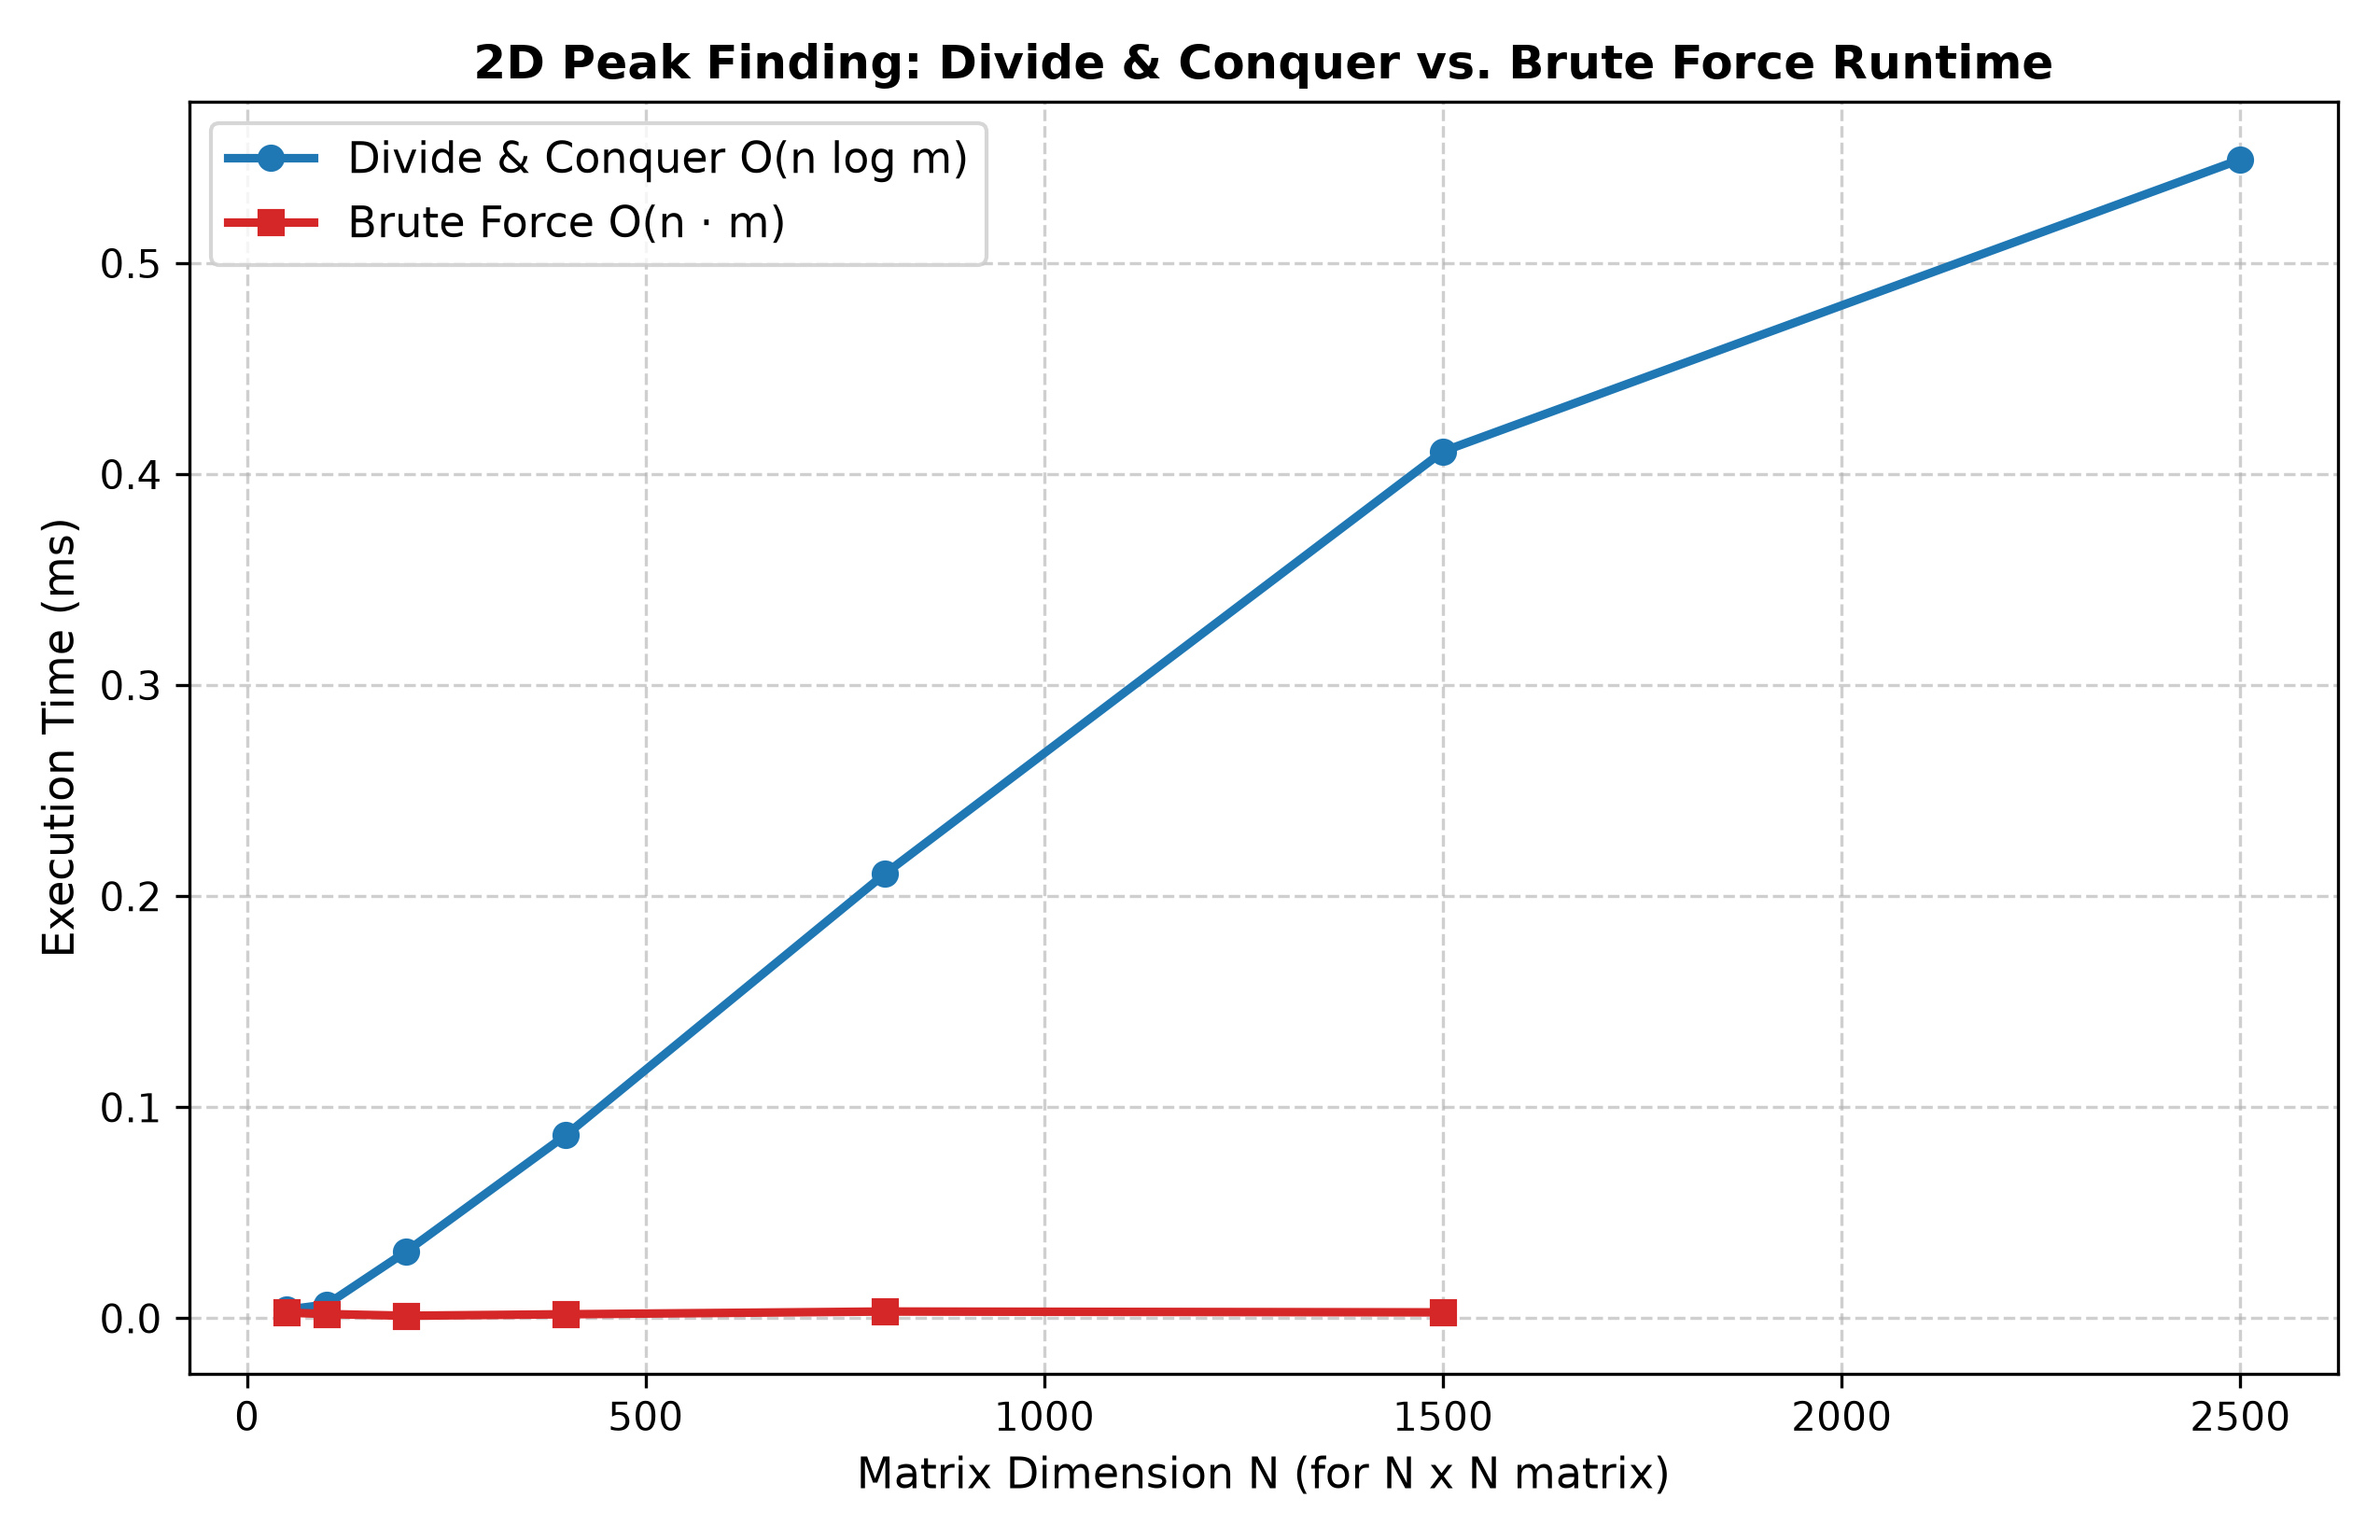
\includegraphics[width=0.75\textwidth]{images/peak_finding_2d_analysis.png}
\caption{Runtime Scaling of 2D Peak Finding via Column Divide and Conquer.}
\label{fig:peak_finding}
\end{figure}

\end{document}
